\documentclass{beamer}
\usepackage[utf8]{inputenc}
\usepackage{graphicx}
\usepackage{color}
%\usetheme{Hannover}
\newcommand{\hilight}[1]{\textbf{\textcolor{structure.fg!85}{#1}}}
\setbeamertemplate{footline}[frame number]

\usepackage{hyperref}
\hypersetup{
    colorlinks=true,
    linkcolor=blue,
    filecolor=magenta,      
    urlcolor=cyan,
}

\author[Sowmya Vajjala]{Sowmya Vajjala}

\title[SfSNLP]{NLP without Annotated Dataset}
\subtitle{NLP Careers}


\date{29 January 2021}

\institute{Seminar f\"ur Sprachwissenschaft, University of T\"ubingen, Germany}
%%%%%%%%%%%%%%%%%%%%%%%%%%%

\begin{document}

\begin{frame}\titlepage
\end{frame}

\begin{frame}{Why now?}
    "Perhaps one topic that could be covered is company expectations when hiring and where things stand industry-wise."
\end{frame}

\begin{frame}{I will try to ... }
give a quick overview of... 
    \begin{itemize}
        \item the kind of jobs out there
        \item typical expectations, interview processes
        \item how to keep track of what is going on
    \end{itemize}
    ... based on my very limited knowledge of north american practices, but to German students!
\end{frame}

\begin{frame}{Typical career paths SfS}
(that I know of)
    \begin{itemize}
        \item Getting into a PhD program 
        \item Joining IBM, Mercedes etc. (tech. companies, with potentially NLP work)
        \item Joining translation services companies (e.g., Transline in Reutlingen) 
        \item Joining in general software engineer roles
        \item Linguist roles in tech companies or related ones
    \end{itemize}
    (SfS alumni are into all of these, in and outside Germany. Try to reach out for help/referrals!)
\end{frame}

\begin{frame}{SfS Alumni}
... are at:
    \begin{itemize}
        \item IBM, Amazon, Elastic (Elastic Search), Microsoft
        \item Mercedes, Daimler, Volkswagen
        \item Software AG
        \item Transline (at least used to be)
        \item Almato, GFai, Docyet, Carmeq etc
        \item Explosion.AI (Spacy)
    \end{itemize}
\end{frame}

\begin{frame}{Expectations: PhD applications}
    \begin{itemize}
        \item Some background working in research projects
        \item General interest in pursuing research, reading up papers etc
        \item Some ideas to pursue research on
        \item Good written and spoken communication
        \item Reasonbably good programming skills.
    \end{itemize}
\end{frame}

\begin{frame}{PhD life}
\begin{itemize}
    \item Some course work (optional)
    \item work as a research assistant in some funded project
    \item think about what related problem can you solve for phd thesis
    \item write papers
    \item read papers
    \item give talks, attend conferences etc.
\end{itemize}
\end{frame}

\begin{frame}{Expectations: Linguist Roles}
    \begin{itemize}
        \item I have no direct idea.
        \item Companies like Appen have roles for linguists, focusing on data annotation.
        \item Companies like Grammarly have roles involving rule engineering (which needs some linguistics knowledge)
        \item Duolingo has some roles related to language learning exercises 
        \item Google, Microsoft etc all hire linguists for data annotation, evaluation, error analysis kind of profiles
    \end{itemize}
    note: I know these through past students who applied to such positions. No direct experience.
\end{frame}

\begin{frame}{Expectations: Tech companies}
(for NLP projects)
    \begin{itemize}
        \item Very good programming skills (which language is often not too important)
        \item Problem solving skills: how do you approach a problem? 
        \item Some understanding of Linguistics, NLP, Machine Learning, Deep Learning. 
        \item Some prior experience working on some NLP research project
    \end{itemize}
\end{frame}

\begin{frame}{Expectations: Software Engineer roles}
(more generic than the previous slide)
    \begin{itemize}
        \item Very good programming skills.
        \item Ability to convert requirements to code
        \item Ability to understand and follow good coding practices (version control, code review, code profiling, documentation etc)
        \item Learn and adapt quickly
    \end{itemize}
\end{frame}

\begin{frame}{Life in a company}
    \begin{itemize}
        \item Initial years: you may write a lot of code every day, attend some meetings, probably read a lot
        \item mid-years: reduced coding, more design, more meetings, probably some presentations, conferences etc.
        \item later: further reduced hands on work, and more management work. 
    \end{itemize}
\end{frame}

\begin{frame}{What interviewers may look for in companies}
What I look for, when I interview: 
   %advice for junior ds
   \begin{itemize}
       \item Can this candidate explain their course projects clearly?
       \item If I pose a similar (but not same) problem, can they propose a solution, relating this to those problems?
       \item If I ask for an alternative solution, can they think and give some ideas?
       \item Do they have some idea about different "methods", as well as different "application" scenarios, based on course work? 
   \end{itemize}
\end{frame}

\begin{frame}{Specific Skills to prepare for}
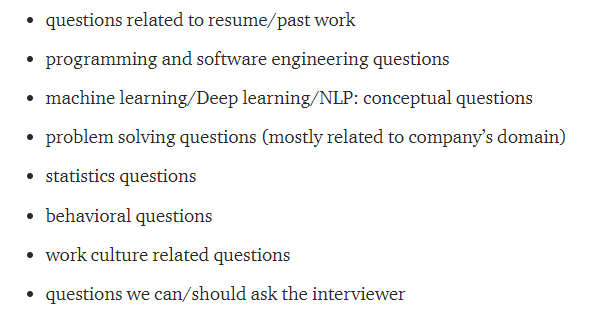
\includegraphics[width=\textwidth]{figures/interviews.PNG}
\href{https://towardsdatascience.com/preparing-for-in-person-data-science-interviews-some-thoughts-5e2677ee30d9}{Source - my blog post about my own job search}
\end{frame}

\begin{frame}{General Notes}
    \begin{itemize}
        \item Good programming skills are a must when starting out. Practice on websites like hackerrank. 
        \item Be willing to keep learning and adapting to change more, at least in initial years out of Uni. 
        \item Don't stick to NLP - see where else can you apply what you learnt in school and apply there too. 
        \item It is useful to have a github profile with some project codes etc. if possible
    \end{itemize}
\end{frame}

\begin{frame}{Useful links}
    \begin{itemize}
        \item \url{https://nlppeople.com/} - I used to look here for jobs.
        \item Twitter - following NLP companies, researchers provide good source of information about current trends, job openings, careers etc.
        \item I follow newsletter.ruder.io (among others) for getting news about recent NLP research updates
        \item TowardsDataScience blog for more practical articles (how to use a library to do X etc)
    \end{itemize}
\end{frame}

\end{document}